\chapter{Introdução}

Um dos problemas enfrentados por pessoas com deficiência motora é a falta de acesso à informação devido à impossibilidade ou dificuldade para usar dispositivos eletrônicos. Uma possível solução para esse problema seria usar o movimento dos olhos para interagir com o mundo exterior. O uso de técnicas para identificar onde determinada pessoa está olhando é chamado de rastreamento de olhar.

\begin{figure}
\centering
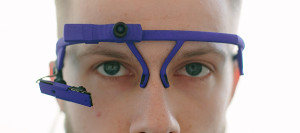
\includegraphics[scale=1]{imagens/dmk-headset.jpg}
\caption{\newc{Exemplo de câmera usada para rastreamento de olhar. Uma câmera posicionada na frente do olho direito registra imagens do olho, que serão usadas para estimar o olhar. Reproduzido de \small{\protect \url{https://pupil-labs.com/blog/2016-07/new-headset-color/}} } }
\label{fig:cam_olho}
\end{figure}

Para rastrear o olhar geralmente uma câmera é posicionada na frente de um dos olhos, \newc{como mostra a Figura $\ref{fig:cam_olho}$}. A partir da imagem obtida pela câmera, técnicas de processamento de imagens são usadas para identificar a posição da pupila e, a partir disso, identificar a direção em que o usuário está olhando. No entanto, o rastreamento de olhar é dificultado por vários fatores, como mudanças na iluminação do lugar e oclusão parcial dos olhos causada por alguma expressão facial. Portanto, não é uma tarefa trivial mas, apesar dessas dificuldades, deve ser executada em tempo real.

Em vez de localizar a pupila na imagem, podemos comparar cada nova imagem do olho com as amostras, ou seja, com imagens do olho correspondendo a diferentes posições de olhar registradas durante a calibração. Podemos encontrar as amostras mais parecidas com a imagem e depois estimar o olhar como uma média ponderada do olhar nas amostras.

Uma imagem em escala de cinza do olho pode ser escrita como uma combinação linear das amostras mais um ruído, representado como uma combinação linear da base canônica de espaço vetorial (onde cada elemento da base pode ser interpretado como uma imagem que é preta em todos os \textit{pixels}, exceto em um). Note que a combinação linear não é única, pois é possível calcular qualquer vetor como combinação linear dos elementos da base.

\newc{Quando a} imagem é muito mais parecida com as amostras do que qualquer vetor da base, assumimos que ela pode ser escrita como uma combinação linear das amostras mais o ruído, onde os coeficientes do ruído são próximos de zero.

Podemos então procurar o vetor de coeficientes com o maior de número de coeficientes nulos. Essa é a abordagem sugerida pelo Compressive Sensing (CS). Chamamos de esparso um sinal que depende apenas de uma pequena quantidade de vetores da base. Quando o sinal depende de vários vetores, chamamos de \textit{compressive}.

Desenvolvemos um programa de rastreamento de olhar usando \textit{Compressive Sensing} e concluímos que esse rastreador apresenta resultado semelhante a \newc{rastreadores comerciais}.